%!TEX TS-program = xelatex
\documentclass[]{friggeri-cv}
\usepackage{afterpage}
\usepackage{hyperref}
\usepackage{color}
\usepackage{xcolor}
\usepackage{smartdiagram}
\usepackage{fontspec}
\usepackage{graphicx}
\usepackage{subcaption}


% if you want to add fontawesome package
% you need to compile the tex file with LuaLaTeX
% References:
%   http://texdoc.net/texmf-dist/doc/latex/fontawesome/fontawesome.pdf
%   https://www.ctan.org/tex-archive/fonts/fontawesome?lang=en
%\usepackage{fontawesome}
\usepackage{metalogo}
\usepackage{dtklogos}
\usepackage[utf8]{inputenc}
\usepackage{tikz}
\usetikzlibrary{mindmap,shadows}
\hypersetup{
    pdftitle={},
    pdfauthor={},
    pdfsubject={},
    pdfkeywords={},
    colorlinks=false,           % no lik border color
    allbordercolors=white       % white border color for all
}
\smartdiagramset{
    bubble center node font = \footnotesize,
    bubble node font = \footnotesize,
    % specifies the minimum size of the bubble center node
    bubble center node size = 0.5cm,
    %  specifies the minimum size of the bubbles
    bubble node size = 0.4cm,
    % specifies which is the distance among the bubble center node and the other bubbles
    distance center/other bubbles = 0.29cm,
    % sets the distance from the text to the border of the bubble center node
    distance text center bubble = 0.28cm,
    % set center bubble color
    bubble center node color = pblue,
    % define the list of colors usable in the diagram
    set color list = {lightgray, materialcyan, orange, green, materialorange, materialteal, materialamber, materialindigo, materialgreen, materiallime},
    % sets the opacity at which the bubbles are shown
    bubble fill opacity = 0.6,
    % sets the opacity at which the bubble text is shown
    bubble text opacity = 0.5,
}

\addbibresource{bibliography.bib}
\RequirePackage{xcolor}
\definecolor{pblue}{HTML}{0395DE}

\begin{document}
\header{SiThu}{Thwin}
      {SRE Team Lead and Solution Architect}

% Fake text to add separator
\fcolorbox{white}{gray}{\parbox{\dimexpr\textwidth-2\fboxsep-2\fboxrule}{%
.....
}}
%...

% Add badges
\begin{figure}[h]
  \centering
  \begin{subfigure}[b]{0.1\linewidth}
    
\includegraphics[width=\linewidth]{img/cka.png}
  \end{subfigure}
  \begin{subfigure}[b]{0.1\linewidth}
    
\includegraphics[width=\linewidth]{img/istio-expert.png}
  \end{subfigure}
  \begin{subfigure}[b]{0.1\linewidth}
    
\includegraphics[width=\linewidth]{img/istio-intermediate.png}
  \end{subfigure}
  \begin{subfigure}[b]{0.1\linewidth}
    
\includegraphics[width=\linewidth]{img/istio-fundamentals.png}
  \end{subfigure}
  \begin{subfigure}[b]{0.1\linewidth}
    
\includegraphics[width=\linewidth]{img/envoy.png}
  \end{subfigure}
  \begin{subfigure}[b]{0.1\linewidth}
    
\includegraphics[width=\linewidth]{img/ccna.png}
  \end{subfigure}
\end{figure}
%...

% In the aside, each new line forces a line break
\begin{aside}
  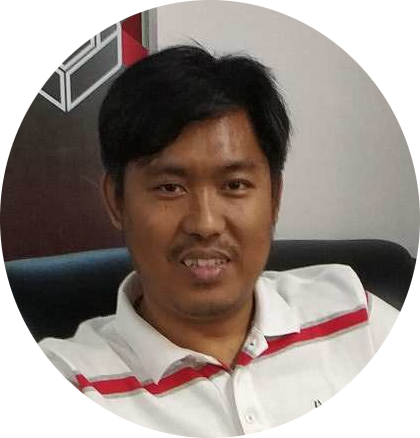
\includegraphics[scale=1]{img/myself-circle.png}
  \section{Traits}
    Quick Learner
    Innovative
  \section{Address}
    CL1-202, Cityloft@Starcity
    Than Lyin Township
    Yangon, Myanmar
    ~
  \section{Contact}
    \textbf{Tel:} +95 979 7969695
    \textbf{Skype:} live:sithuthwin
    ~
  \section{Mail}
    \href{mailto:sithu@thwin.net}{\textbf{sithu@}thwin.net}
    ~
  \section{Social}
    \textbf{LinkedIn:} \href{https://www.linkedin.com/in/si-thu-thwin/}{si-thu-thwin}
    ~
  \section{Web \& Git}
    \href{https://www.thwin.net}{thwin.net}
    \href{https://github.com/herzcthu}{github.com/herzcthu}
    \href{https://gitlab.com/herzcthu}{gitlab.com/herzcthu}
    ~
  % use  \hspace{} or \vspace{} to change bubble size, if needed
  \section{DevSecOps}
    \textbf{GitLab CI/CD}
    \textbf{Terraform/Ansible}
    \textbf{SonarQube}
    \textbf{Maven}
    \textbf{Docker}
    \textbf{ELK/EFK}
    \textbf{Prometheus/Grafana}
    \textbf{K8S/Openshift/Helm/Istio/Single Mesh}
    \textbf{Pinpoint/Zipkin}
    \textbf{PHP}
    \textbf{Python/Flask}
    \textbf{YAML}
    \textbf{Bash}
    \textbf{LaTeX}
    \textbf{gRPC/mTLS/PKI}
    \textbf{AWS/Azure/Oracle}
    \textbf{MySQL/MongoDB}
    ~
\end{aside}
~
%...

\section{Experience}
\begin{entrylist}
  \entry
    {Aug/20 - Now}
    {SRE team Lead and Solution Architect}
    {YOMA Bank}
    { \begin{itemize}
      \item Responsible for administering of 6 Kubernetes clusters in hybrid cloud enviornment.
      \item Responsible for developing DevOps CI/CD pipeline.
      \item Maintain ISTIO service mesh in hybrid cloud Kubernetes enviornment.
      \item Responsible for managing resources on Azure cloud.
      \item Maintain and manage RHSSO, Keycloak, WSO2 APIM.
      \item Responsible for administering Kafka Cluster and MongodB Cluster.
      \item Manage VMWare infrastructure. Administrator for Databases such as Mysql, Mongodb, PGsql.
      \item Leading the team with engineers responsible for VMWare, Azure Cloud, Kubernetes, Oracle, Linux, various applications in banking enviornment.
      \item Solution Architect for various applications and systems such as Mobile Banking application.
      \end{itemize}
    }
  \entry
    {Mar/19 - Aug/20}
    {Lead DevOps Engineer}
    {YOMA Bank}
    { \begin{itemize}
        \item Lead DevOps in Digital Transformation. Responsible for building CI/CD pipeline and Training DevOps Engineers.
        \item Maintain Digital Banking application backend services which include IBM Websphere, Active MQ, Oracle DB.
        \item Maintain Core Banking and lead the team responsible for maintainance of the all application in bank system.
      \end{itemize}
    }
  \entry
    {Aug/17 - Mar/19}
    {Assistant Team Lead (System and Database)}
    {YOMA Bank}
    {
      \begin{itemize}
        \item Oracle and MySql management.
        \item Responsible for daily maintainance of Databases. Improving database and system performance. I have successfully improved 7 hour long DB backup process to complete within 20 Minutes.
      \end{itemize}
    }
  \entry
    {Apr/16 - Aug/17}
    {Senior System Administrator}
    {Blue Ocean Call Center}
    {
      \begin{itemize}
        \item Manage SIP Gateway, Asterisk, VMware, UCS server, SIP routing.
        \item Responsible for all hardware/software in the whole Data Center with 4 Racks and 10 ESXi Servers.
        \item Adding/installing/configuring for ESXi Servers, Dell EMC servers.
        \item Setting up Databases, Web Servers, Applications Servers.
        \item Develop PHP based applications required for the company. Such as small CRM application.
      \end{itemize}
      }
\end{entrylist}

\section{Skills}
\begin{entrylist}
  \entry
  {Microservices}
  {Kubernetes, Helm, Keycloak, WSO2 APIM, RHSSO}
  {DevOps}
  {  \begin{itemize}
      \item Expert in Kubernetes Cluster Management. CI/CD pipeline developments. DevOps and NFR tooling.
      \item Proficient with Kubernetes and developing Helm charts
      \item Maintain Keycloak, RHSSO and WSO2 APIM. Have fundamentals knowledge of IAM and APIs.
      \item Applicable knowledge and experienced about API and Restful standards.
    \end{itemize}}
    \entry
    {System Engineering}
    {Linux, Windows Servers, Cloud, VMWare}
    {DevOps}
    {  \begin{itemize}
        \item Expert in Linux.
        \item Well experienced Windows system administration.
        \item More than 7 years experienced in working on AWS and Digital ocean. More than 4 years working on Azure Cloud.
        \item Experience with VCenter management, SAN storage management. Good knowledge with TCP/IP network stacks.
      \end{itemize}}
  \entry
  {Service Mesh}
  {ISTIO, Single Mesh, Service Discovery}
  {DevOps}
  {  \begin{itemize}
      \item Very well experienced with ISTIO, mTLS, Service Mesh
    \end{itemize}}
  \entry
  {Messaging}
  {Kafka, ActiveMQ, Strimzi, Debezium}
  {DevOps}
  { \begin{itemize}
      \item Manage and configure Kafka, CDC, MQ
    \end{itemize}}
  \entry
  {CI/CD}
  {GitOps, GitFlow, Gitlab, Tools Integration, APM, NFR}
  {DevOps}
  { \begin{itemize}
      \item git operation and gitflow, Jenkin, Jira, SonarQube
      \item Can work with any DevOps tools used for NFR infrastructure
      \item Grafana, Prometheus, Jaeger, Zabbix, Pinpoint, Graylog
    \end{itemize}}
  \entry
  {Database}
  {Oracle, MySQL, MongoDB, SQL}
  {DBA}
  { \begin{itemize}
      \item SQL Language, Oracle RAC cluster, RMAN, Dataguard, MongoDB cluster, MySQL clusters
    \end{itemize}}
  
\end{entrylist}


\section{Certifications and Degree}
\begin{entrylist}
  \entry
  {01/2023}
  {CKA}
  {cncf.io}
  {\emph{Certified Kubernetes Administrator}}
  \entry
  {04/2019}
  {LinuxFoundationX - LFS158x}
  {edx.org}
  {\emph{Introduction to Kubernetes}}
  \entry
  {09/2014}
  {CCNA Cisco Certified Network Associate}
  {PearsonVUE}
  {\emph{Routing and Switching}}
  \entry
  {2001 - 2004}
  {Bachelor's Degree in German Language}
  {UFL, Mandalay}
  {Specialized in German Language\\ }
  
\end{entrylist}

\section{Other Experiences and Professions}
~
\begin{entrylist}
  \entry
  {Trainer}
  {Trainer for DevSecOps Engineering}
  {BIM Training}
  {Teach and train for DevSecOps Engineering classes}
  \entry
  {Mentorship}
  {Mentor for CS50}
  {Personal}
  {Personal mentor for CS50 - Introduction to computer science}
  \entry
  {Consultant}
  {ICT Consultant for Election Monitoring}
  {NDI, Washinton DC}
  {Develop data collection software (Web based and SMS). Data syncronization between cloud and local server. This software is used in 
    \begin{itemize}
      \item 2015 General Election Myanmar
      \item 2017 By-Election Myanmar
      \item 2017 General Election Cambodia
      \item 2020 General Election Myanmar
    \end{itemize}}
  \entry
  {Cloud}
  {DataCenter Migration}
  {blueplanet.com.mm}
  {
    \begin{itemize}
      \item Move on-prem datacenter to AWS cloud. Auto scaling EC2 instances using spot instance. 
      \item Data replication between on-prem and cloud. Asterisk SIP routing from cloud to on-prem servers.
    \end{itemize}}
\end{entrylist}

\begin{aside}
~
~
~
~
  \section{Referee}
    \textbf{Sander Meinema}
    \href{mailto:sander@architectingasaservice.com}{\textbf{sander@}architectingasaservice.com}
  ~
  \section{Personal Skills}
  \smartdiagram[bubble diagram]{
    \textbf{Quick}\\\textbf{Learner},
    \textbf{Organize},
    \textbf{Team}\\\textbf{Player},
    \textbf{Initiative},
    \textbf{Curiosity},
    \textbf{Problem}\\\textbf{Solving},
    \textbf{Manage}
  }
~
\end{aside}
\section{Training}
\begin{entrylist}
  \entry
  {Self-Paced}
  {LFS258 Kubernetes Fundamentals}
  {linuxfoundation.org}
  {Certified Kubernetes Administrator Program}
  \entry
  {09/2018}
  {RedHat Openshift Workshop}
  {RedHat}
  {\emph{Openshift setup on-prem with Ansible. Openshift Architecture}}	\entry
  {07/2018}
  {VMware Certified Professional 6.5}
  {BIM Training, VMware Official}
  {\emph{Datacenter Virtualization}}
  \entry
  {09/2014}
  {Advanced Network Engineering}
  {RHC Technologies}
  {\emph{Advanced networking. Routing and switching}}
\end{entrylist}

\textbf{\emph{March 20th, 2023}}
\hfill
\textbf{\emph{Sithu Thwin}}
\end{document}